%\documentclass[aps,pra,reprint,longbibliography]{revtex4-1}
\documentclass[twocolumn]{article}

\usepackage{geometry}
\geometry{textwidth = 18cm,textheight = 24cm}

%\usepackage{multicol}
\usepackage{caption}

\usepackage{graphicx}
\usepackage{amsmath}
\usepackage{float}
%\usepackage{amssymb}
\usepackage{textcomp}
%\usepackage{lmodern}
\newenvironment{figure_alt}
  {\par\medskip\noindent\minipage{\linewidth}}
  {\endminipage\par\medskip}

\begin{document}
	
	%-------------------- begin header -------------------%
	\centerline{\LARGE Optoelectronic Intelligence}%Light in neural systems%Intelligent optoelectronic systems
	\vspace{0.75em}
	\centerline{\Large Jeffrey M. Shainline}
	%\vspace{0.75em}
	%\centerline{\large National Institute of Standards and Technology}
	\vspace{0.5em}
	\centerline{\large NIST, Boulder, CO, 80305}
	\vspace{0.5em}
	\centerline{\large \today}
	%-------------------- end header ---------------------%
	
\begin{abstract}
We motivate the design of optoelectronic neural systems based on principles of neuroscience and very-large-scale integration. We argue that for large neural systems capable of general intelligence, the strengths of photonics for communication and electronics for computation are indispensable. Based on these considerations, we sketch a concept for optoelectronic hardware, beginning with synaptic circuits and extending to systems at the scale of the human brain and beyond.
\end{abstract}

\section{\label{sec:introduction}Introduction}
Light is excellent for communication. Fiber optic links carry vast quantities of information across continents and between data centers. An important question in modern computing is: what is the shortest distance over which photonic communication will displace electronic interconnects? Optical links between racks in data centers are becoming common. Major companies are investing seriously in photonics in the package. Monolithic optical links between processor and memory fabricated in a 45-nm CMOS node with no in-line changes have been demonstrated \cite{suwa2015}. A primary challenge affecting further chip-scale electronic-photonic integration is the continued difficulty of achieving a light source implemented on silicon that is robust, efficient, and economical.

In parallel with the hardware considerations affecting optoelectronic integration are questions related to architecture. A prominent theme emerging as we approach the end of conventional scaling is parallelism. Computation is increasingly distributed among more processor cores. Many-core architectures continue to expand into on-chip networks, in some cases resulting in highly distributed, brain-inspired systems \cite{bo2000,pfgr2013,mear2014,fuga2014,payu2017,dasr2018}. As compute grows more distributed, communication across interconnection networks becomes a bottleneck. The demand for energy efficient communication bandwidth has been a major driver of on-chip photonics.

The major drivers for brain-inspired computers fall on a spectrum: energy and algorithmic efficiency for deployable applications reside on one side of the spectrum, and artificial general intelligence (AGI) resides on the other. Knowledge gained from neuroscience informs us that systems with general intelligence will benefit from very large numbers of computational elements as well as extreme communication between them. It is our perspective that hardware incorporating light for communication between electronic computational elements combined with an architecture of distributed optoelectronic spiking neurons will provide tremendous potential for AGI. Considerations pertinent to the realization of such a technology are the subject of this article.

\section{\label{sec:sructureAndFunction}Structure and function across space and time}
\begin{figure*} 
    \centering{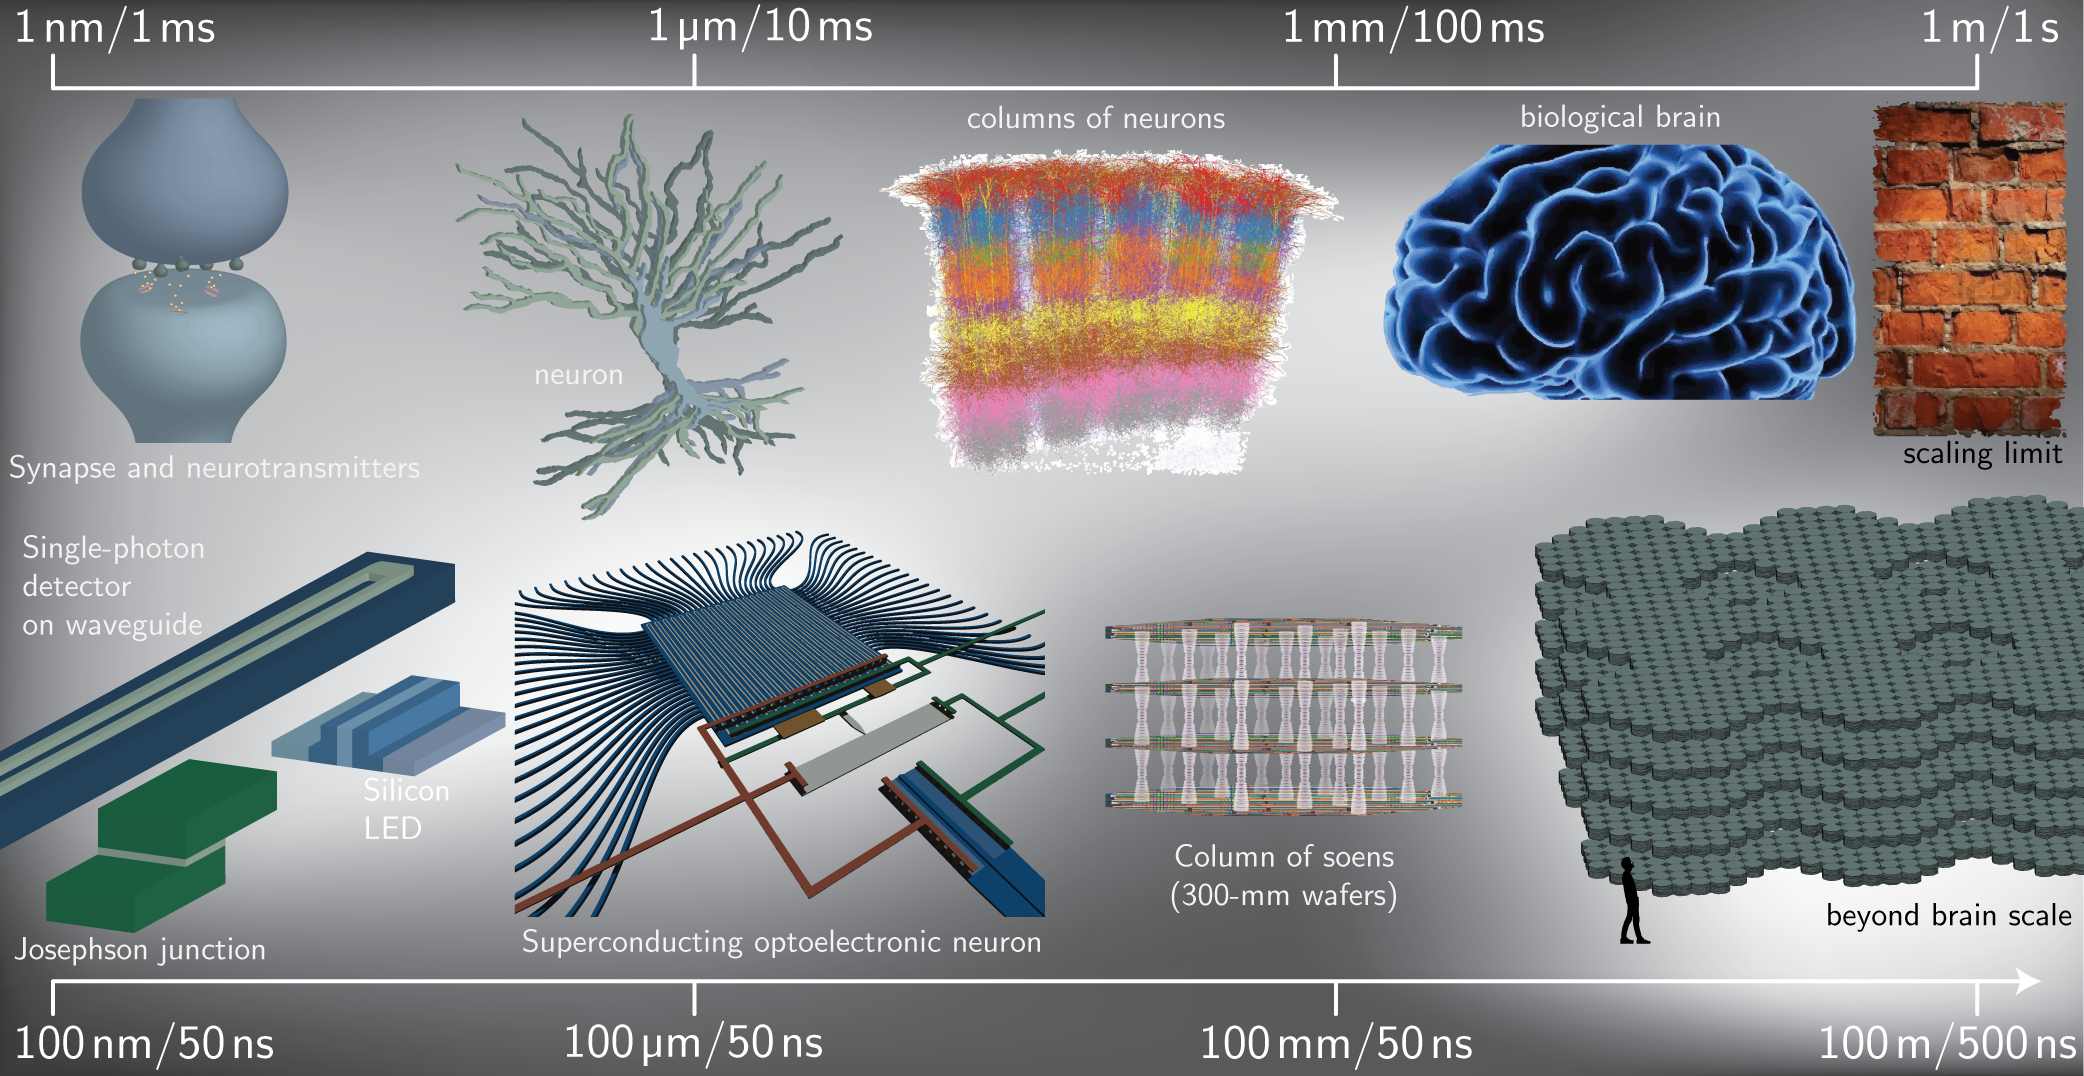
\includegraphics[width=17.2cm]{complexity_across_scales.png}}
	\captionof{figure}{\label{fig:complexityAcrossScales}Complexity across scales. (add temporal scales to axes)}
\end{figure*}
To guide the design of hardware for AGI, we must simultaneously consider operation across spatial and temporal scales. In Fig.\,\ref{fig:complexityAcrossScales}, we chart the structures present on various length scales and temporal scales for biological and optoelectronic hardware. The human brain has features spanning roughly eight orders of magnitude in size, from a nanometer to a tenth of a meter, with correlated dynamical activity across four orders of magnitude, from below 1\,Hz to around 600\,Hz. There are several types of optoelectronic neural systems, and we have proposed a specific approach we see as most conducive to large-scale implementation for AGI \cite{sh2018}. These optoelectronic networks are likely to have features as small as 100\,nm and potentially extend up to many kilometers. Dynamical activity may be present from slow temporal scales up to 20\,MHz (30,000 times the maximum speed of the brain) for networks measured in kilometers. To enable such spatial and temporal scaling, fractal properties must be employed.

Information processing in neural systems employs local clusters of neurons to represent specific features, and the information from these clusters must be shared with other regions of the network to form a multifaceted representation of a complex stimulus. Structurally, this information processing is facilitated by networks with a high clustering coefficient yet also an average path length nearly as short as a random graph \cite{eskn2015}. Such graph structures are referred to as small-world networks \cite{wast1998}, and are ubiquitous throughout the brain \cite{sp2010}. To achieve small world networks, long-range connections are necessary. In a random network, near and distant connections are equally probable, so the average path length across the network is small, representing a lower limit on path length for a given number of edges connecting a given number of nodes. In Fig.\,\ref{fig:data}(a) we plot the number of edges required per node to achieve a given average path length as a function of the number of nodes in the network \cite{frfr2004}. Consider the case of a network with one million nodes. We see from this plot that if we wish to maintain a path length of two, each node must make, on average, one thousand connections. For the case of a network with 100 million nodes, each node must make 10,000 connections. This is similar to the case of the hippocampus in the human brain, with nearly 100 million neurons, each with 10,000 or more synaptic connections. Maintaining a short average path length across the network is critical to enable efficient information integration, and this appears to be a major factor driving the extensive connectivity of biological neural systems. In the present context, this motivates us to conceive of artificial hardware capable of supporting comparable connectivity, which leads us to consider using light for communication.
\begin{figure} 
    \centering{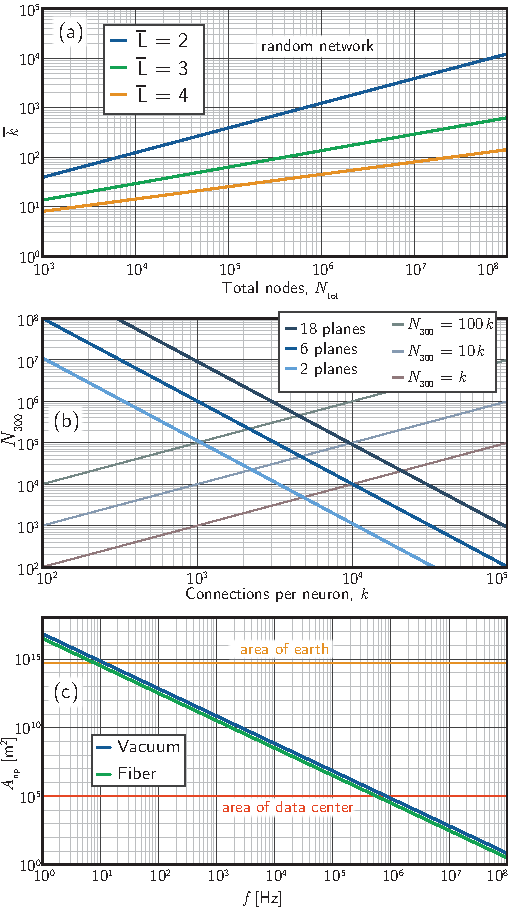
\includegraphics[width=8.6cm]{data_plots.pdf}}
	\captionof{figure}{\label{fig:data}Data plots.}
\end{figure}

In addition to structural considerations pertinent to information integration across space, we must also consider how information propagates across time in neural systems. The computational primitives best equipped to integrate information across space and time are neurons, relaxation oscillators that encode information in the timing of their pulses. One of the most impressive aspects of neural information processing is that the same structural network can be used at different times in different contexts to form myriad functional networks. Over time scales on the order of neuronal inter-spike intervals, this is accomplished in two ways. First, short-term synaptic plasticity enables synapses to rapidly adapt in response to network activity, essentially resulting in temporal filtering of afferent spike trains \cite{abre2004}. Second, inhibitory neurons working in conjunction with dendrites can silence or give voice to specific synapses, clusters of synapses, or neurons depending on the local and global activity of the network. In addition, dendritic processing, wherein the dendritic arbor performs intermediate, nonlinear transformations between synapses and the soma, enables utilization of timing information \cite{vagu2005}, detection of sequences of activity \cite{haah2015}. Over time scales long compared to an average inter-spike interval, long-term potentiation and depression of synapses is employed to store memories and adapt the network to a small-world architecture \cite{shki2006}. Learning in the presence of a continually changing environment while maintaining long-term memories is achieved through spike-timing-dependent plasticity (STDP) \cite{somi2000,mage2012} and metaplasticity \cite{ab2008,fudr2005}. Neurons employing inhibition, dendritic processing, short-term, and long-term synaptic plasticity can make efficient use of a structural network by dynamically adapting on time scales from an inter-spike interval to the lifetime of the system. We refer to these synaptic, dendritic, and neuronal functions collectively as the computations performed by the neurons, and the standard threshold/spike operation is included. While light is excellent for communication with high fan-out between neurons in a cluster as well as across distant regions of a network, electrical circuits are better equipped to perform the computations necessary for adapting a vast structural network into dynamical functional networks useful for information processing. 

In neural information processing, space and time are interrelated. This is evident both in oscillatory behavior such as cross-frequency coupling as well as anharmonic behavior such as neuronal avalanches. Cross-frequency coupling enables fast activity of local clusters to be modulated and sampled on slower time scales across larger regions of the network \cite{stsa2000,heze2010}. Cross-frequency coupling is enhanced during activities that require attention and coordinated response of multiple brain regions, and is one technique by which the brain utilizes oscillations at various frequencies for information integration \cite{bu2006}. Neuronal avalanches, on the other hand, are present as background activity even when attention is not directed to a particular subject, and can be anharmonic in nature \cite{heze2010}. Yet, similar to cross-frequency coupling, such cascades of spiking activity communicate across local, regional, and global partitions of the network. We denote by $s$ the number neurons involved in a neuronal avalanche. Neural activity across many species, brain regions, and contexts shows the probability of observing an avalanche of size $s$ follows a power law: $P(s)\sim s^{-\alpha}$. Systems with a power-law distribution of neuronal avalanches demonstrate self-organized criticality \cite{plth2006}, which maximizes the dynamic range of the system \cite{kico2006,be2007}. Such a power-law dependence has the important property that the ratio of number of events of size $qs$ to the number of events of size $s$ is simply $q^{-\alpha}$, independent of $s$. For this reason, such a distribution is referred to as ``scale-free'', and is self-similar, or fractal, across spatial and temporal scales. 

Related to the fractal scaling of neuronal avalanches, neural systems are fractal in space in that they obey power-law scaling of connectivity \cite{bagr2010}, as well as in time in that they demonstrate power-law power-spectral density \cite{budr2004}. Fractal properties of neural systems are crucial to operation. Fractal systems can continue to scale, with dynamics constrained only by the physical hardware and spatial extent of the system rather than by the ability to communicate across the architecture \cite{plth2007}. Such scale-free systems can efficiently integrate information from local clusters to vast networks, while enabling correlations across wide regions of space and long periods of time. We conjecture that intelligent systems must achieve small-world structural networks with many nodes, and the computational elements comprising the nodes must support adaptive, dynamical responses on many time scales to fully utilize the structural networks for functional computation. We further conjecture that light is most capable of achieving communication across the structure of the network, while electronic circuits are most capable of achieving the dynamical activity necessary for computation. Based on these consideration, we expect a hardware platform capable of AGI to combine the strengths of photonic communication with electronic computation to integrate information in neuronal avalanches from small, local clusters on a silicon wafer to the light-cone-limited region of space across which light can travel in a network oscillation cycle.  

\section{\label{sec:synapsesDendritesAndNeurons}Optoelectronic synapses, dendrites, and neurons}
The device factors mentioned above are not quirks of the biological world, but rather are some of the reasons brain computation is so complex and efficient. Short-term plasticity produces information about spike train rising and falling edges and guards against runaway activity. STDP strengthens correlations between neurons that fire constructively and dampens connections that waste energy. These mechanisms have been shown to adapt random structural networks into complex functional networks with small-world architecture and neuronal avalanches indicating maximal dynamic range due to criticality. Dendritic processing in conjunction with inhibitory interneurons makes efficient use of the complex spatial network by dynamically activating a wide range of functional networks. To achieve these myriad computational functions, optical interactions are inadequate. The complexity of electronic circuits is required. 

We envision optoelectronic hardware with photonic communication along waveguides playing the role of axons, and computation performed in electronic synapses, dendrites, and neurons. We make two more choices to specify the platform. Detectors must respond to single photons for maximal energy efficiency. Superconducting-nanowire single-photon detectors (SNSPDs) are the clear choice for this application, with very low dark counts, near-zero static power dissipation, and scalable integration \cite{shbu2017b}. An SNSPD is simply a current-biased strip of superconducting wire roughly 100\,nm in width and 5\,nm in thickness. SNSPD operation is summarized as follows. In the steady state, the current bias flows straight to ground, and upon detection of a photon, a small section of the wire is driven from the superconducting phase to the normal-metal phase, resulting in a transient resistance of a few kiloohms for a few hundred picoseconds. This resistance produces a transient current bias to a load. 

In addition to the choice of SNSPDs as the detectors in the system, we must also select a light source, which must be fabricated across wafers by the millions for economical, brain-scale systems. Because our choice of detectors dictates cryogenic operation, silicon light sources operating at 4\,K are an option \cite{da1989,shxu2007}. This neural system may be one of the few applications where silicon light sources are appropriate and sufficient. The light sources we have in mind are silicon LEDs \cite{buch2017}, employing luminescence from defect-based dipole emitters \cite{dali1987,absa2018}. From the perspective of VLSI, achievement of a silicon light source of sufficient performance would be the greatest contribution to the success of this technology. If cryogenic operation enables both single-photon detectors and silicon light sources, it will almost certainly be worth the effort.

To achieve complex neural circuits, we must combine light sources, detectors, and various other circuit elements. We have demonstrated waveguide coupling of light from these micron-scale light sources to integrated SNSPDs on a silicon photonic chip \cite{buch2017}. The detectors can be engineered in circuits with Josephson junctions (JJs) and superconducting loops coupled through mutual inductors to achieve the functions we need for neural information processing. Candidate circuit designs have been presented in Refs.\,\cite{sh2018b,sh2018c,sh2018d,sh2018}, and much more innovation is certainly possible. In optoelectronic synapses of this design, the current bias across a single JJ establishes the synaptic weight. This current bias can be modified through various photonic and electronic means based on network activity. Inhibition is straightforward with opposing mutual inductors. Dendritic and neuronal nonlinearities are a natural consequence of the fact that Josephson junctions have a critical current. The extreme nonlinearity of the superconducting phase transition plays a leading role for both for the generation of light during a neuronal firing event and the detection of light at synapses. Due to the prominent role of superconducting current storage loops, we refer to these as loop neurons. In the operation of loop neurons, a single photon triggers a synaptic event, and STDP is induced by two photons\textemdash one from each neuron associated with the synapse.

\section{\label{sec:communication}Communication with guided light}
The central premise of our work is that photonic signals are superior to electronic signals for communication across large-scale neural systems. To explain why we place this conjecture at the center of hardware development, we briefly summarize the physical limitations of electrical interconnection networks \cite{hepa2012}. It is impracticable in silicon electronics for a single device to source current to many other devices. A shared communication network must be employed. In contemporary computing, switched media networks are used for this purpose. Each device must then only communicate to the nearest switch in the network. The interconnect network determines a valid route for the information to traverse across the network, and the switches are configured accordingly. Because the communication infrastructure is shared, devices must request access to the switch network to transmit messages. When multiple devices request access simultaneously, arbitration must be performed, wherein devices are queued and sequentially granted access to the switch network. This approach to communication between electronic devices leverages the speed of electronic circuits to compensate for the difficulties in communication. The limitations are reached when many devices need to communicate with many other devices with a high frequency of communication events. Unfortunately, this is exactly the situation encountered in neural information processing. During a neuronal avalanche, many neurons may need to communicate simultaneously across the network. As more neurons, each with many synapses, are added to the network, the average frequency of neuronal firing events must decrease due to the limitations of the interconnection network to handle communication requests, and large neuronal avalanches integrating information across the network cannot be supported by the communication infrastructure.

The physics of light is complimentary to that of electrons. Photons, being uncharged bosons, interact very weakly with each other. Thus, in the linear regime in which this few-photon technology will operate, photons can co-propagate on waveguides independently of one another without wiring capacitance. This enables a pulse of photons to fan out to many destinations without a charging penalty due to wiring. This is not to say photonic communication can address an arbitrarily large number of recipients without consequence. For each new recipient, the number of photons in the initial pulse must increase, and as destinations get further away, more energy is dissipated to propagation loss. These realities notwithstanding, it appears feasible for devices communicating with photons to make direct connections to thousands of destinations, thereby eliminating the need for the shared communication infrastructure that is the primary impediment to achieving AGI with electrical interconnections.

Having made this claim, the burden is upon us to provide evidence of the feasibility of photonic communication in large-scale neural systems. Much like electrical interconnection networks utilize different technologies at the scales of chips versus data centers, photonic interconnection technologies will vary at different scales to enable communication in chip-scale systems as well as across networks the size of a data center. The small-world architectures displaying Rentian scaling that are suitable for neural information processing require neurons to communicate seamlessly across all scales of network hierarchy. The large wavelength of light relative to the size of electronic devices (and relative to the size of devices in the brain) cause concern for the size of optoelectronic brain-scale networks. To build confidence for the feasibility of the endeavor, we sketch a vision of how a general optoelectronic neural system may be constructed.

A successful neural technology must leverage the fabrication infrastructure of silicon electronics. We conjecture that silicon photonics technology will be utilized to move light between neurons. At the wafer scale, light will be guided in dielectric waveguides. Silicon photonics provides three primary dielectric materials that can be used for these passive waveguides: Si, SiN, and SiO$_2$. The indices of refraction of these materials are 3.5, 2.0, and 1.5, respectively, for $\lambda$ close to 1550\,nm. Perhaps not coincidentally, these are the three primary dielectrics used in CMOS technology as well. Achieving the dense routing required to connect large numbers of neurons on a wafer will require multiple planes of waveguides, just as integrated electronics requires multiple wiring layers. We anticipate optoelectronic neural systems will utilize dielectric waveguide layers deposited in the back-end-of-line in the fabrication process, with lower layers having higher index and being utilized for local connections, and higher layers having gradually lower index with lower propagation loss used for more distant connections. 

We wish to approximate the area of such photonic interconnection networks. Following Keyes \cite{ke1982}, we approximate the area required for the waveguides entering a neuron as $A_{\mathrm{n}} = (n_{\mathrm{in}} w/k)^2$, where $n_{\mathrm{in}}$ is the number of waveguides entering the neuron (in-directed synaptic connections), $w$ is the waveguide pitch, and $k$ is the number of planes of waveguides. In general, $w$ will depend on index contrast, but for this analysis we approximate it as constant and utilize an intermediate value. For tiling multi-wafer assemblies, wafers diced into octagons may be advantageous, so we take the area of a wafer to be $A_8 = 2\sqrt{2}r^2$ with $r = 150$\,mm. The number of neurons that can be supported on a 300-mm wafer is given by the ratio,
\begin{equation}
\label{eq:numNeuronPerWafer}
N_8 = \frac{A_8}{A_{\mathrm{n}}} = 2\sqrt{2}r^2\left(\frac{k}{wn_{\mathrm{in}}}\right)^2.
\end{equation}
This expression is plotted in Fig.\,\ref{fig:data}(b). This estimate informs us that a 300 mm wafer with six waveguide planes can support roughly one million neurons if they each have one thousand connections. More involved analysis finds a slightly smaller number \cite{sh2018e}. As a point of comparison to electrical neural systems, Ref.\,\cite{kuwa2017} finds that through multi-layer, wafer-scale integration of logic and memory, 250 million electrical neurons could fit on a 300-mm wafer. The trade-off is speed, as the shared communication network would limit the electrical neurons studied in Ref.\,\ref{kuwa2017} to 10\,Hz operation. Nevertheless, the message of Fig.\,\ref{fig:data}(b) is that photonic routing results in large area consumption. The human cortex contains over 10 billion neurons. An optoelectronic brain larger than a bumble bee will not fit on a wafer.

\begin{figure*}[] 
	\centering{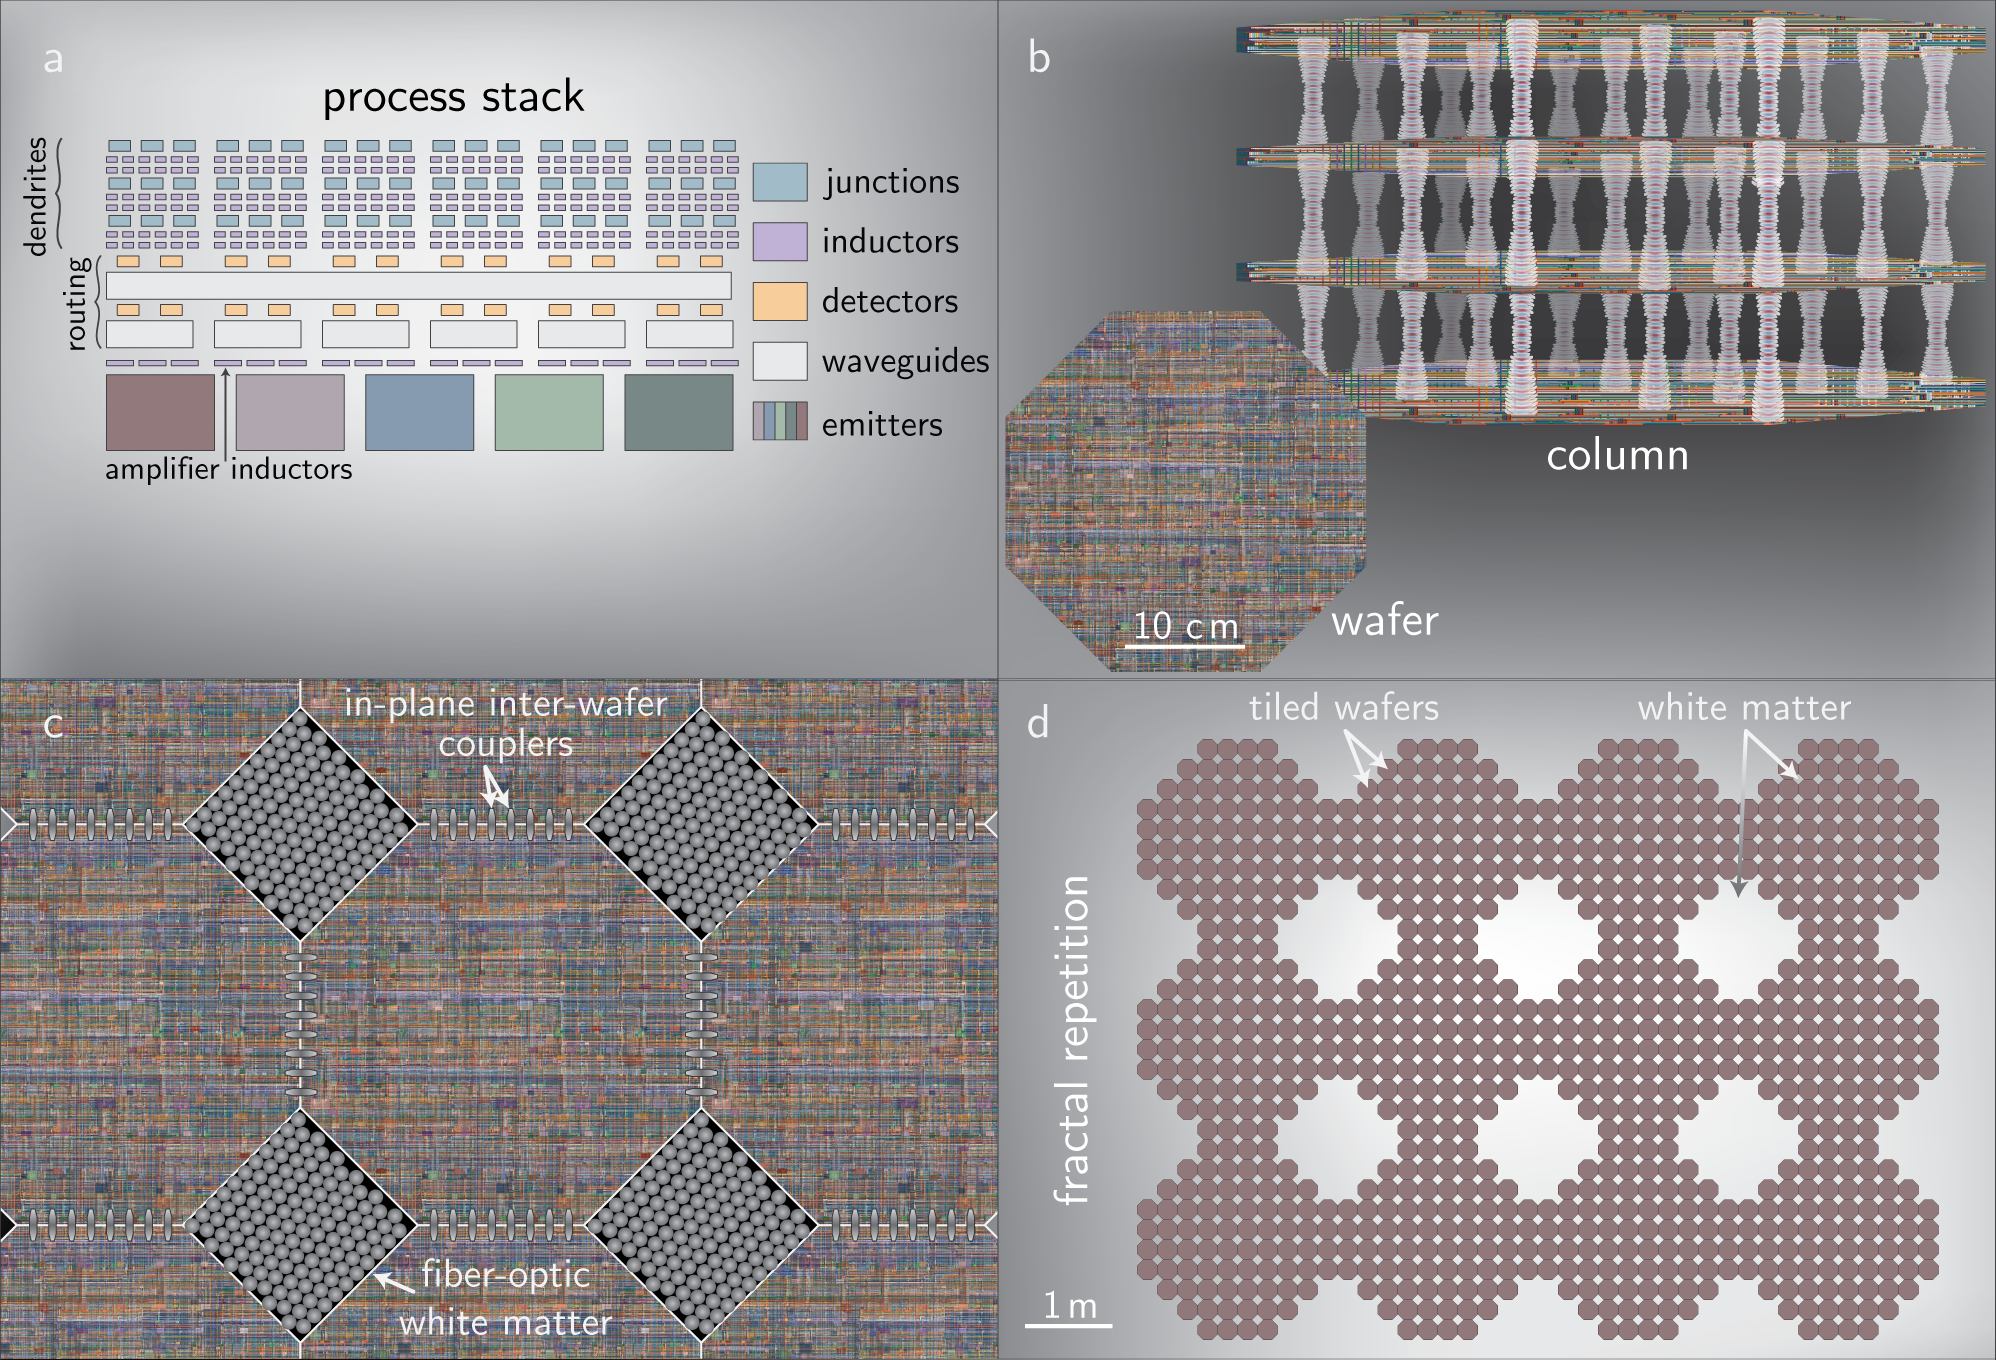
\includegraphics[width=14cm]{communication_across_scales.png}}
	\captionof{figure}{\label{fig:communicationScales}Photonic interconnection on various length scales.}
\end{figure*}
Optoelectronic intelligence will require communication between wafers. Wafers can be stacked vertically, and free-space optical links can send photons from a source on one wafer to a detector on a wafer above or below, as illustrated in Fig.\,\ref{fig:communicationScales}(a). Such 3D wafer-stacking techniques are being developed for electronics, but the ability of light to propagate through free space (or liquid helium) and the ten-micron alignment tolerances enabled by wide-area photodetectors \cite{mave2013} make such 3D integration promising for photonic communication as well. Assuming SNSPDs receiving vertical communication have a pitch of 25\,\textmu m, a 300-mm octagon could support $10^8$ vertical communication links between two wafers. Assuming half of this area is for feed-forward communication from the lower wafer to the upper wafer, and half is for feed-back from the upper wafer to the lower wafer. This would result in $5\times10^7$ synaptic connections originating from neurons on one wafer and terminating in neurons on a vertically adjacent wafer. If each wafer had one million neurons with one thousand connections per neuron within the wafer, the total number of intra-wafer synaptic connections would be $10^9$. Therefore, the number of synapses present in a layer of this network that originated on a previous layer would be 5\%, similar to the fraction observed in the laminar structure of biological cortex (Ref.\,\cite{bu2006}, pg. 286).

In addition to free-space vertical coupling, inter-wafer communication can be achieved at wafer edges with in-plane waveguide couplers, as shown in Fig.\,\ref{fig:communicationScales}(c). In the octagonal (truncated square) tiling used here for illustration, each wafer makes such connections to neighbors in the cardinal directions. With a 10\,\textmu m pitch, 11,500 wafer-edge couplers could be supported in each of the cardinal directions with 46,000 total in-plane, lateral connections. Such a system would demonstrate strong connectivity within the vertical stack of the wafers, and weaker lateral connectivity between wafers in the same horizontal plane. Such an architecture resembles the columnar organization of cortex.  

The wafer tiling we have just described leads to a picture of optoelectronic networks with vertically stacked columns of wafers with horizontal connectivity emanating from the perimeter of each wafer. To achieve communication from within these columns to other (perhaps distant) regions of the network, optical fibers are ideal. Within the truncated square tiling under consideration, the square areas at diagonals between wafers can support fiber-optic bundles. These optical fiber tracts are analogous to white matter in the brain. One such region could house a million standard single-mode fibers of 125\,\textmu m diameter. These fibers will emanate from all wafers within the column, so the number of outputs available to each wafer will depend on how many vertically integrated wafers are utilized in a column. If six wafers are stacked in a column, each wafer would have roughly 167,000 output fibers to carry information to distant regions of the network. With one million neurons on a wafer, this would mean not every neuron on the wafer would be able to couple to a fiber for long-distance communication. This again is consistent with brain organization wherein the number of long-distance axons emanating from a region is smaller than the number of neurons within the region. Note, however, that each of these fibers can branch as it propagates through the white matter, so a neuron with access to a single wafer-edge fiber could establish multiple long-range synaptic connections. 

On a wafer, photonic fan-out across dielectric waveguides enables neurons to make thousands of direct connections without the limits of a shared switching network. Free-space and wafer-edge couplers enable significant inter-wafer communication conducive to columnar information processing. Such columns can communicate to one another locally and globally over fiber optic links. With this configuration in mind, we can assess the feasibility of constructing systems on the scale of the human cerebreal cortex, with 10 billion neurons, each with thousands of synaptic connections. If a wafer holds a million neurons, a brain-scale assembly requires 10,000 wafers and would fit in a volume two meters on a side\textemdash the size of a few server racks in a closet. 

We are optimistic that this approach to neural information processing will be successful for physical and practical reasons. Physically, due to photonic signaling, it is possible to achieve efficient communication across the network for systems with orders of magnitude more than 10,000 wafers. As we see in Fig.\,\ref{fig:data}(c), networks with activity at 1\,MHz can span an area hundreds of meters on a side before communication delays limit the speed of network activity. Due to superconducting electronics, the power density of such systems will be low enough for liquid helium cooling. On the practical side, fabrication of loop neurons appears at industrial scale appears feasible, because all the proposed circuits can be created on 300\,mm wafers with existing infrastructure, such as a 45\,nm CMOS node. Ten thousand wafers move through such a foundry every day. If dedicated to fabrication of optoelectronic intelligence, a single foundry may be able to produce multiple brain-scale systems per year. Assembly of the wafers into a functional system would be difficult, but probably not more difficult than the construction of a contemporary supercomputer. The requirement of liquid-helium cooling is not a major impediment. Note that no transistors are utilized in loop neurons. The only semiconducting components are the light sources, and all neuronal computations are performed with superconducting electronics. While a VLSI platform combining these light sources with superconducting detectors, thin-film amplifiers, Josephson junctions and passive dielectric waveguides is perhaps even more ambitious than silicon microelectronics, the project has the advantage that it is resilient to device imperfections due to the intended mode of information processing. For example, the exponential dependence of Josephson junction characteristics on tunneling-barrier thickness makes it difficult to yield digital logic circuits based on JJs across a wafer. In the neural application under consideration, some variability can be tolerated \cite{stro2005}, and high connectivity along with synaptic plasticity are likely to compensate for device variation.

The greatest unknown is the source of light. If silicon sources that have already been demonstrated in cryogenic optical links \cite{buch2017} can be produced with internal quantum efficiency $\eta_{\mathrm{qe}}\approx 10^{-3}$, we anticipate this project will be economically viable. At present, $\eta_{\mathrm{qe}} = 5\times10^{-7}$ has been demonstrated in the first attempt with no optimization of optical or electrical properties. For the superconducting optoelectronic neural systems described here, the light sources need not achieve high performance. They are only required to produce incoherent pulses of roughly 10,000 photons ($\approx 1$\,fJ) at 20\,MHz. If no silicon light source operating at 4\,K can meet these criteria, and integration of III-V light sources on silicon wafers is required, the cost and complexity of a project at this scale may become prohibitive.

\section{\label{sec:discussion}Discussion}
At present, the challenge of creating an artificial intelligence rivaling a human appears formidable with the use of silicon electronics alone. The primary challenge arises because direct signaling between large numbers of neurons is not possible due to the charging requirements of wires and devices, so shared communication infrastructure is required, resulting in a connectivity/speed tradeoff. The use of photonic communication will mitigate this tradeoff, despite the increased size of photonic interconnection networks. Photonic fanout enables direct connections between large numbers of neurons, and the velocity of light enables communication across ten-meter systems before communication limits network speed below the 20\,MHz where loop neurons are limited by electronic reset times. 

Light is excellent for communication, while electronics excel at computation. Artificial neural hardware should be designed and constructed to leverage photonic communication while performing synaptic, dendritic, and neuronal functions with electronic circuits for computation. Superconducting optoelectronic circuits appear to naturally implement these functions, in part because light sources and detectors work much better at low temperature, and in part because of the utility of Josephson nonlinearities for neural computation. This hardware differs in important ways from the silicon transistors that implement Boolean logic in the framewor of the von Neumann architecture. But such digital computers emerged to perform arithmetic calculations in a manner based on a Turing machine. Neural information processing departs markedly from the sequential operation of a Turing apparatus, so we should not be surprised that optimal hardware may differ as well. Yet for the superconducting optoelectronic hardware discussed here, the fabrication infrastructure is largely the same as contemporary CMOS. We see this hardware and computing application as an instance where light sources and detectors can and must be densely integrated for communication between primitive compute nodes (neurons), yet distant communication is also optical, primarily in fiber-optic waveguides, thereby simultaneously leveraging the strengths of integrated silicon photonics as well as fiber-optic networks.

What are the next steps to realize this technology? Low-cost source-detector integration at the wafer scale is required. These active devices must be augmented with improvements in deposited dielectrics for photonic routing to enable more planes with lower loss. For system scaling, improved fiber-to-waveguide coupling and multi-wafer modules must be demonstrated. All the hardware improvements will not lead to AGI without further theoretical analysis at device, circuit, and system levels. Further understanding the principles of network information processing and designing the architecture to achieve general intelligence are likely to be much more challenging than understanding the operation of a Turing machine. Theoretical progress is required to understand how to implement functional systems, train them, and make them intelligent.

\bibliographystyle{abbrv}
\bibliography{optoelectronic_intelligence}

\end{document}